% -*- coding: utf-8 -*-
\documentclass[compress,usepdftitle=false,xcolor=pdftex,dvipsnames,table,aspectratio=169]{beamer}
\usepackage{appendixnumberbeamer}% End page count before \appendix
\usepackage{etex}
\usepackage[utf8]{inputenc} % The encoding
%\usepackage[11pt]{moresize}% More font sizes
\usepackage{eulervm}% Euler VM as math serif font

\usepackage{etoolbox}% Needed for toggles

%%%%%%%%%%%%%%%%%%%%%%%%%%%%%%%%%%%%%%%%%%%%%%%%%%%%%%%%%%%%%%%%%%%%%%%%%%%%%%%
%% Setup
%%% The bibliography
% \usepackage[style=authoryear]{biblatex}
% \bibliography{scalas-rebac-ref-rev}

\usepackage{amsmath}
%\usepackage{mathabx} % Beware: may cause compilation problems
\def\rightSquigarrow{\mathrel{\mathlarger{\mathlarger{\rightsquigarrow}}}}
\usepackage{stmaryrd}
%\usepackage{cmll} % \bigwith
% \usepackage{figlatex} % Adds .fig support for \includegraphics

%\usepackage{multirow}
\usepackage{nicefrac}               % Nice fractions
%\usepackage{colonequals} % More symbols (colon equalities)
\usepackage{multirow}% Multirows in tables

\usepackage{relsize} % Relative scaling of text/math

%\usepackage{fixltx2e} % Text mode subscript and superscript
\usepackage{xspace} % Smart spaces after commands
\usepackage{xifthen} % Extended conditional commands

%\usepackage{MnSymbol}% \llangle, \rrangle and other parentheses & symbols
\usepackage{pifont}% Fancy dingbats

\usepackage{tikz}                   % For comic-like balloons
\usetikzlibrary{matrix, positioning, shapes, arrows,
  decorations.markings, automata}
% \usetikzlibrary{calc,shapes.callouts,shapes.arrows}

\usepackage[absolute,overlay]{textpos} % Absolute placement of blocks

%\usepackage[inference]{semantic}    % Helper package for semantics
\usepackage{proof}                  % Logic proofs

\usepackage{ulem} % For strikeout effect
%\usepackage{listings}

\usepackage{transparent} % Transparent text (e.g. in Inkscape-generated images)

% \usepackage{verbatim}

% \usepackage{wasysym} % for smileys

\usepackage{pdfpages}% To include pages from an external PDF file

\usepackage{mathtools} % \xRightArrow and stuff - load late to avoid conflicts

% % Comic-like balloons, arrows etc.
% \newcommand{\arrowthis}[2]{
%         \tikz[remember picture,baseline]{\node[anchor=base,inner sep=0,outer sep=0]%
%         (#1) {{#1}};
%         \node[overlay,single arrow,draw=none,fill=red!50,anchor=tip,rotate=60] 
%         at (#1.south) {#2};}%
%     }%
% \newcommand{\bubblethis}[2]{
%         \tikz[remember picture,baseline]{\node[anchor=base,inner sep=0,outer sep=0]%
%         (#1) {{#1}};\node[overlay,cloud callout,callout relative pointer={(0.2cm,-0.7cm)},%
%         aspect=2.5,fill=yellow!90] at ($(#1.north)+(-0.5cm,1.6cm)$) {#2};}%
%     }%
% \newcommand{\speechthis}[2]{
%         \tikz[remember picture,baseline]{\node[anchor=base,inner sep=0,outer sep=0]%
%         (#1) {{#1}};\node[overlay,ellipse callout,fill=blue!50] 
%         at ($(#1.north)+(-.5cm,0.8cm)$) {#2};}%
%     }%
% \newcommand{\pointthis}[2]{
%         \tikz[remember picture,baseline]{\node[anchor=base,inner sep=0,outer sep=0]%
%         (#1) {{#1}};\node[overlay,rectangle callout,%
%         callout relative pointer={(0.2cm,0.7cm)},fill=green!50] at ($(#1.north)+(-.5cm,-1.4cm)$) {#2};}%
%         }%

%%%%%%%%%%%%%%%%%%%%%%%%%%%%%%%%%%%%%%%%%%%%%%%%%%%%%%%%%%%%%%%%%%%%%%%%%%%%%%%
% Workaround to make \pause behave correctly inside alignments
%
% See:
%
% http://tex.stackexchange.com/questions/6348/problem-with-beamers-pause-in-alignments
%%%%%%%%%%%%%%%%%%%%%%%%%%%%%%%%%%%%%%%%%%%%%%%%%%%%%%%%%%%%%%%%%%%%%%%%%%%%%%
\makeatletter
\def\beamerorig@set@color{%
  \pdfliteral{\current@color}%
  \aftergroup\reset@color
}
\def\beamerorig@reset@color{\pdfliteral{\current@color}}
\makeatother
%%%%%%%%%%%%%%%%%%%%%%%%%%%%%%%%%%%%%%%%%%%%%%%%%%%%%%%%%%%%%%%%%%%%%%%%%%%%%%%

% Highlighting
\newcommand{\HLight}[1]{{\setlength{\fboxsep}{0pt}\colorbox{yellow}{#1}}}
\newcommand{\HLightB}[1]{{\setlength{\fboxsep}{0pt}\colorbox{Lavender!50}{#1}}}
% \newcommand{\OKLight}[1]{{\setlength{\fboxsep}{0pt}\colorbox{green}{#1}}}
% \newcommand{\KOLight}[1]{{\setlength{\fboxsep}{0pt}\colorbox{gray}{#1}}}
\newcommand{\OKmark}{\ensuremath{{\huge{\color{Green}\text{\ding{51}}}}}}%
\newcommand{\KOmark}{\ensuremath{{\huge{\color{Red}\text{\ding{55}}}}}}%
\newcommand{\smallOKmark}{\ensuremath{{\Large{\color{Green}\text{\ding{51}}}}}}%

\definecolor{hlight}{rgb}{0.99, 0.95, 0.80}
\setbeamercolor{hlightBox}{bg=hlight}
\setbeamercolor{yellowBox}{bg=yellow}

\newcommand{\bluebf}[1]{{\textbf{\color{blue}#1}}}%
\newcommand{\redbf}[1]{{\textbf{\color{red}#1}}}%
\newcommand{\greenbf}[1]{{\textbf{\color{OliveGreen}#1}}}%
\newcommand{\brownbf}[1]{{\textbf{\color{Brown}#1}}}%

% Horizontal separator
\newcommand{\myRule}{%
  \vspace{-0.3cm}
  {\color{Gray}\rule{\textwidth}{1pt}}
  \vspace{-0.2cm}
}%

% Strikeout
\newcommand\redout{%
  \bgroup\markoverwith{\textcolor{Red}{\rule[0.4ex]{10pt}{4pt}}}\ULon%
}

%\usetheme[subsection=false]{Dresden}
\useoutertheme[subsection=false]{miniframes}
\usefonttheme{professionalfonts}
\setbeamercolor{section in head/foot}{fg=white, bg=black}
% \setbeamercolor{mini frame}{fg=white, bg=black}
\usefonttheme[onlylarge]{structurebold}
%\setbeamerfont*{frametitle}{size=\normalsize,series=\bfseries}
\setbeamertemplate{navigation symbols}{}
%\setbeamertemplate{headline}[miniframes theme]{}
%\setbeamertemplate{footline}[default]
\setbeamertemplate{footline}[frame number]

%%\usecolortheme{whale}

%\setbeamercovered{transparent=20}

\normalem % Don't mess with \em and \emph!

%% Squeeze bibliography style
\setbeamertemplate{bibliography entry title}{}
\setbeamertemplate{bibliography entry location}{}
\setbeamertemplate{bibliography entry note}{}

%\usepackage{fancyvrb}% Required by pygments.tex below
%\input{pygments.tex}% Autogenerated by Makefile

%% Macro definitions
\input{macros.tex}
%x\newcommand{\putat}[3]{\begin{picture}(0,0)(0,0)\put(#1,#2){#3}\end{picture}}

%%%%%%%%%%%%%%%%%%%%%%%%%%%%%%%%%%%%%%%%%%%%%%%%%%%%%%%%%%%%%%%%%%%%%%%%%%%%%%%
%% Title
\def\myTitlePlain{Dynamic formation of the distributed\\ $\mu$ clouds}%
\def\myTitle{Dynamic formation of the distributed\\ $\mu$ clouds}

\hypersetup{
  pdfauthor={Milo\v s Simi\' c},
  pdftitle={\myTitlePlain},
  pdfkeywords= {cloud computing} {distributed systems} {micro clouds} {distributed clouds},
}

\title{%
  \\[8mm]%
  \huge%
  \myTitle%
}%

\institute[University of Novi Sad, Serbia]{}

\author{%
  \vspace{-1mm}%
  \centering%
   {Milo\v s Simi\'c}\\%
   \vspace{3mm}%
   \centering%
   {{\bluebf{--- Ph. D. Thesis ---}}}%
  \quad
  \\[7mm]%
  \scalebox{0.8}{%
  \begin{minipage}{1.2\linewidth}
  \centering%
  %\raisebox{-6mm}{%
    \includegraphics[height=12mm]{images/novi-sad.pdf}%
    \raisebox{2mm}{
      \begin{minipage}[b]{0.30\linewidth}
        \bf%
        University of Novi Sad\\
        Faculty of Technical Sciences
      \end{minipage}
    }% end \raisebox
  \end{minipage}
  }% end \scalebox
  \vspace{-0mm}%
}% end \author

\date{%
}% end \date

\newcommand{\quickCite}[1]{{\scriptsize\color{gray}(#1)}}

%%%%%%%%%%%%%%%%%%%%%%%%%%%%%%%%%%%%%%%%%%%%%%%%%%%%%%%%%%%%%%%%%%%%%%%%%%%%%%%

 

\begin{document}

\frame[plain]{%
  \titlepage%
}

\setcounter{framenumber}{0}%

\section{Intro}%
\subsection{Intro}%

\begin{frame}
	\frametitle{Table of contents}
	
	\begin{itemize}
		\item Research questions
		\item Cloud computing infrastructure and its problems
		\item Distributed clouds and micro clouds model
		\item Conclusion
		\item Future work
	\end{itemize}
	
\end{frame}

\begin{frame}
	\frametitle{Research Questions}
	
	\begin{enumerate}
		\item \textit{Can geo-distributed nodes be organized in a similar  way to the cloud, but adopted for the different environment, with clear separation of concerns and familiar applications model for users forming micro cloud a model?}
		\item \textit{Can these organized nodes, micro clouds, be offered as a service based on the cloud pay as you go model, to the developers and researchers so that they can develop new human-centered applications?}
		\item \textit{Can a model be created in such a way that it is formally correct, easy to extend, understand and reason about?}
	\end{enumerate}
	
\end{frame}

\begin{frame}
	\frametitle{List of publications}
	
	This thesis is the result of research and development, and it is based on the previously presented papers at conferences in journals.
	\newline
	\begin{itemize}
		\item Journal publications:
		\begin{enumerate}
			\item \textbf{Simić M.}, Prokić I., Dedeić J., G. Sladić and Milosavljević B., "Towards Edge Computing as a Service: Dynamic Formation of the Micro Data-Centers," in IEEE Access, vol. 9, pp. 114468-114484, 2021, doi: 10.1109/ACCESS.2021.3104475
			\item \textbf{Simić, M.}; Sladić, G.; Zarić, M.; Markoski, B. Infrastructure as Software in Micro Clouds at the Edge. Sensors 2021, 21, 7001 https://doi.org/10.3390/s21217001
		\end{enumerate}
	\end{itemize}
\end{frame}

\begin{frame}
	\begin{itemize}
		\item Conference papers:
		\begin{enumerate}
			\item \textbf{Simić, M.}, Stojkov, M., Sladić, G., Milosavljević, B.  CRDTs as replication strategy in large-scale edge distributed system: An overview. In: Zdravković, M., Konjović, Z., Trajanović, M. (Eds.) ICIST 2020 Proceedings Vol.1, pp.46-50, 2020, ISBN 978-86-85525-24-7.
			\item \textbf{Simić M.}, Stojkov M., Sladić G., Milosavljević B., Zarić M.:   On container usability in large-scale edge distributed system, 9. International Conference on Information Science and Technology (ICIST), Kopaonik: Society for Information Systems and Computer Networks, 10-13 March, 2019, pp. 97-101, ISBN pp.97-101, 2019.
			\item \textbf{Simić M.}, Stojkov M., Sladić G., Milosavljević B.:  Edge computing system for large-scale distributed sensing systems, 8. International Conference on Information Science and Technology (ICIST), Kopaonik: Society for Information Systems and Computer Networks, 11-14 March, 2018, pp. 36-39, ISBN 978-86-85525-22-3.
			\item \textbf{Simić M.}, Sladić G., Milosavljević B.:  A Case Study IoT and Blockchain Powered Healthcare , 8. PSU-UNS International Conference on Engineering and Technology - ICET, Novi Sad: University of Novi Sad, Faculty of Technical Sciences , 8-10 June, 2017, pp. 1-4, ISBN 978-86-7892-934-2.
		\end{enumerate}
	\end{itemize}
	
\end{frame}

\section{Thesis background}%
\subsection{Thesis background}%

\begin{frame}
	\frametitle{Background}
	
	\begin{itemize}
		\item The entire research in the domain of three main components:
		\begin{enumerate}
			\item \textbf{Distributed systems} and its applications:
			\begin{itemize}
				\item Cloud computing
				\item Big Data
				\item Service-oriented architectures
			\end{itemize}
			\item \textbf{Infrastructure as software} and its applications:
			\begin{itemize}
				\item Automation
				\item Infrastructure abstraction
			\end{itemize}
			\item \textbf{Containers} and their possibilities in software systems
		\end{enumerate}
	\item They are crucial for understanding the concept of \textbf{distributed clouds --- micro clouds}
	\end{itemize}
	
\end{frame}

\begin{frame}
	\frametitle{Distributed systems}
	
	\begin{itemize}
		\item Multiple entities can communicate, but at the same time, they can perform some operations
		\item Interesting assumptions:
		\begin{itemize}
			\item A computing element -- either a hardware device or a software process
			\item Clients believe they are dealing with a single system -- meaining that the nodes need to collaborate
		\end{itemize}
		\item Three significant characteristics are:
		\begin{enumerate}
			\item \textbf{Concurrency} -- multiple activities are executed at the same time on multiple nodes
			\item \textbf{Independent failures} -- nodes fail independently
			\item \textbf{Lack of a global clock} -- each node has its notion of time, no global clock
		\end{enumerate}
	\end{itemize}
	
\end{frame}

\begin{frame}
	\frametitle{Cloud computing}
	
	\begin{columns}
		\begin{column}{0.5\linewidth}
			\begin{center}
				\textbf{Take 1:} pyramid of offered services
				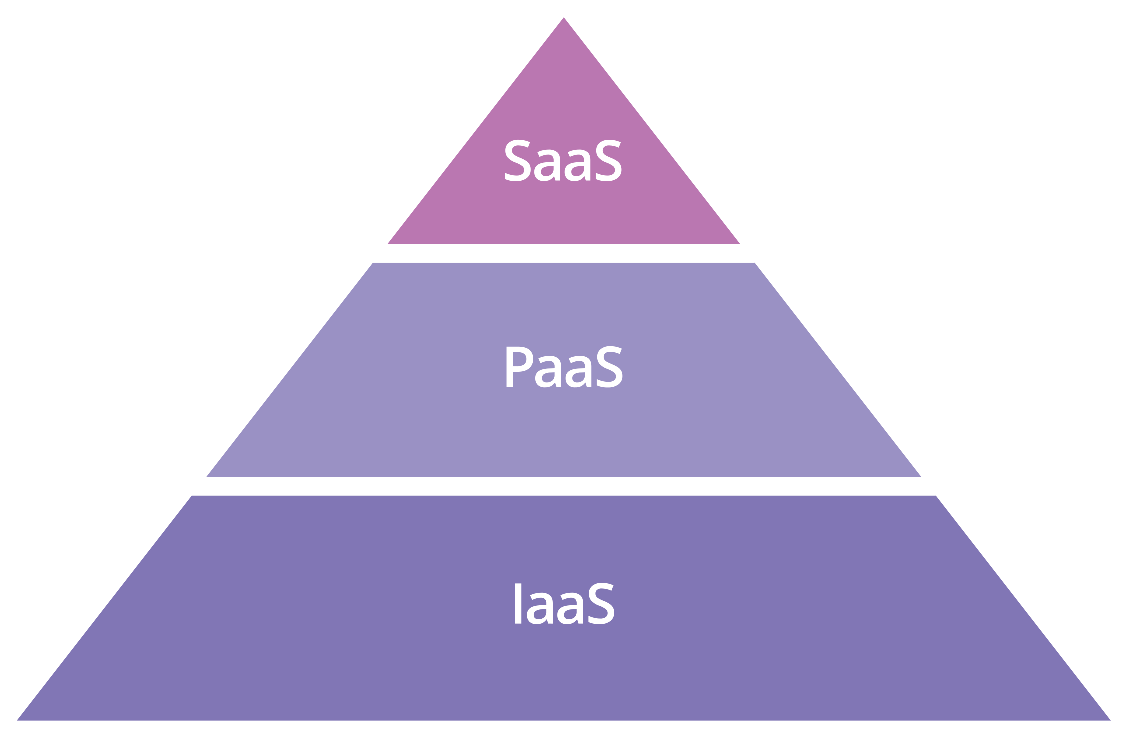
\includegraphics[width=1\linewidth]{images/pyramid}
			\end{center}
		\end{column}
		\begin{column}{0.5\linewidth}
			\begin{center}
				\textbf{Take 2:} favorite provider
				\includegraphics[width=0.73\linewidth]{images/aws}
			\end{center}
		\end{column}
	\end{columns}
	
\end{frame}

\begin{frame}
	\frametitle{What is the cloud then?}
	
	\begin{itemize}
		\item Vogels et al. describe cloud computing as an \textbf{aggregation of computing resources as a utility, and software as a service} --- interesting definition
		\item Clouds provide services, clients use them to avoid huge investments -- creating and maintaining data centers
		\item Pay for their usage time -- \emph{pay as you go model}
		\item Centralization of resources -- \textbf{economy of scale}, lower the administration costs
		\item \textbf{BUT} data \textbf{must} to be moved to the cloud -- \textbf{introduces high latency}
	\end{itemize}
	
\end{frame}

\begin{frame}
	\frametitle{Cloud architecture}
	
	\begin{itemize}
		\item \textbf{Cluster} -- a set of nodes (resources) that operate as a unit to achieve some goal
		\item \textbf{Region} -- a set of clusters, isolated and independent from each other
		\item Regions are usually composed of a few \textbf{availability zones} -- defense against the fail
		\item If one zone fails or goes offline, there are still more of them to serve requests -- better availability, scalability, and resilience
	\end{itemize}
	
	\bigskip
	
	\begin{itemize}
		\item On top, services are built to fully utilize cloud infrastructure
	\end{itemize}
	
\end{frame}

\begin{frame}
	\frametitle{Cloud computing problems}
	
	\begin{itemize}
		\item Centralization demands to move all data to the cloud --- big issue
		\begin{itemize}
			\item Boeing 787s per single flight generates \textbf{half a terabyte of data}
			\item A self-driving car generates \textbf{two petabytes of data per single drive}
		\end{itemize}
		\item Bandwidth is not large enough to support such requirements
		\item Some applications require real-time processing for proper decision-making
		\item Such applications might face \textbf{serious issues} if a cloud service becomes unavailable
		\item Some sensitive data cannot be moved out of the state border
		\item When pushed to its limits, centralization brings more harm than good
	\end{itemize}
	
\end{frame}

\section{Distributed clouds model}%
\subsection{Distributed clouds model}%

\begin{frame}
	\frametitle{Distributed clouds}
	
	\begin{itemize}
		\item The cloud is usually far away from end devices -- data centers are built on specific locations (target as many users nearby as possible)
		\item Sparse deployment will most likely lead to high latency, and bad quality of experience (QoE)
		\item Latency-sensitive applications \textbf{especially} will have a hard time
		\item Relax the cloud, and move some tasks from the cloud -- opening the door for next gen models
		\item Models where computing and storage resources are in \textbf{proximity to data sources}
	\end{itemize}
	
\end{frame}

\begin{frame}
	\frametitle{Next gen}
	
	\begin{columns}
		\begin{column}{0.5\linewidth}
			\begin{center}
				\includegraphics[width=1\linewidth]{images/matrix}\\
				\quickCite{Cloud Native Maturity Matrix}
			\end{center}
		\end{column}
		\begin{column}{0.5\linewidth}
			\begin{center}
				\includegraphics[width=1\linewidth]{images/dgcp}\\
				\quickCite{Google distributed cloud}
			\end{center}
		\end{column}
	\end{columns}
	
\end{frame}

\begin{frame}
	\frametitle{Edge computing}
	
	\begin{itemize}
		\item Edge computing introduced \textbf{small-scale servers} -- operate \textbf{between data sources and the cloud}
		\item These small-scale servers
		\begin{itemize}
			\item Have much fewer capabilities compared to the cloud servers
			\item Operate in proximity to data sources
			\item Maintain good performance to build servers and clusters
		\end{itemize}
		\item To avoid latency and huge bandwidth, edge computing nodes can be dispersed in various locations
		\item Nearby nodes could be \textbf{organized locally} -- \textbf{extending resources beyond the single node or group of nodes}
	\end{itemize}
	
\end{frame}

\begin{frame}
	\frametitle{Related work}
	
	\begin{itemize}
		\item Platform models:
		\begin{itemize}
			\item Kubernetes -- an (updated) open-source variant of Google orchestrator Borg
			\item Nebula
			\item OpenStack
		\end{itemize}
	\item Nodes organization:
	\begin{itemize}
		\item Zone-based organization
		\item Micro data centers -- serve nearby population (theory)
		\item Nano data centers -- serve single household (using SDN)
		\item Drop computing -- ad hoc formation
	\end{itemize}
	\item Processing:
	\begin{itemize}
		\item Data locality -- moving computation to the data
		\item Lambda architectures
	\end{itemize}
	\item Infrastructure definition as code
	\end{itemize}

\end{frame}

\begin{frame}
	\frametitle{Proposal}
	
	\begin{itemize}
		\item The cloud architecture is separated into building blocks making the system easier to understand, maintain and operate -- clusters, regions, availability zones
		\item Rely on a similar proven strategy -- adapt the existing model for different use-cases
		\item Let's observe \textbf{micro clouds} as \emph{geo-distributed systems with dispersed users}
		\item \emph{Geo-distribution} means \textbf{in proximity to some large populations}, where micro clouds serve user requests locally \textbf{first}
		\item Forming micro clouds (pools of resources) depends on usage and local population needs -- \textbf{as code/software}
	\end{itemize}
	
\end{frame}

\begin{frame}
	\frametitle{Organization of the nodes}
	
	\begin{itemize}
		\item A group of nodes virtually and/or geographically separated, working together to provide the same service to clients, forms a \textbf{cluster}
		\item A concept used to describe a set of clusters (that could be) scattered over an arbitrary geographic region, is a \textbf{region}
		\item Highest logical concept that is composed of a minimum of one region and could span over multiple regions is a \textbf{topology}
		\item \textbf{To lower the latency, vast distances between clusters should be strongly avoided in normal circumstances!}
	\end{itemize}
	
	\bigskip
	
	\begin{table}[h!]
		\begin{center}
			\begin{tabular}{l|l}
				\textbf{Edge centric computing} & \textbf{Cloud computing}\\
				\hline
				Topology (logical) & Cloud provider (logical)\\
				Region (logical) & Region (physical)\\
				Cluster (physical) & Zone (physical)\\
			\end{tabular}
		\end{center}
	\end{table}
	
\end{frame}

\begin{frame}
	\frametitle{Separation of concerns}
	
	\begin{figure}[H]
		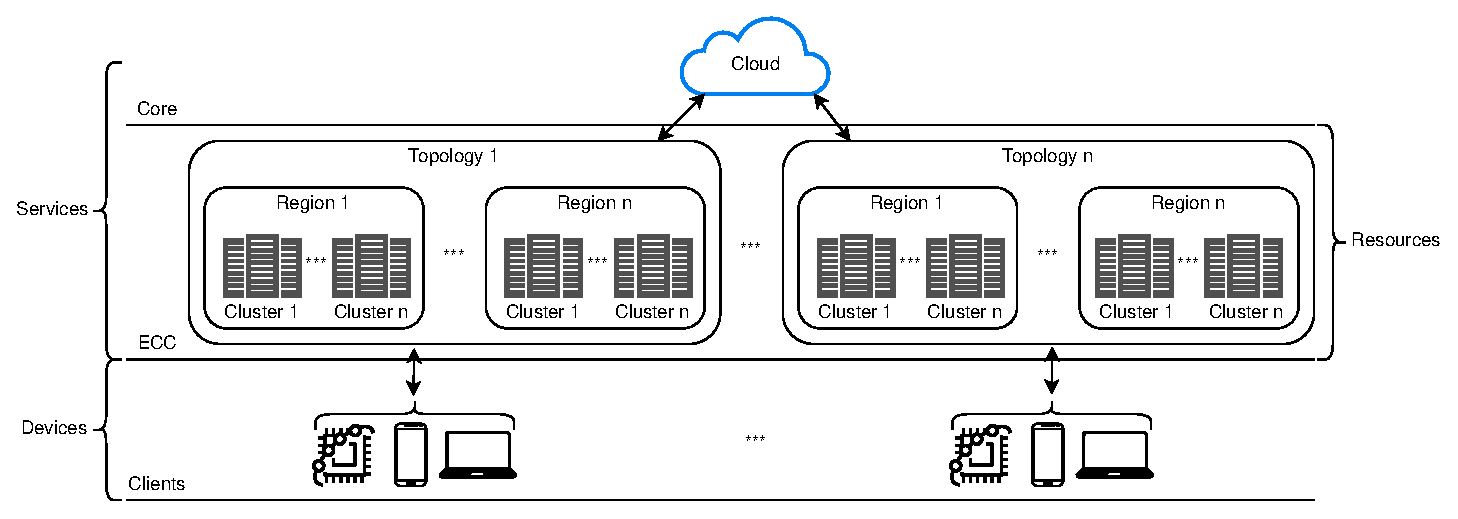
\includegraphics[width=\linewidth]{images/FIG1}
	\end{figure}
\end{frame}

\begin{frame}
	\frametitle{Micro clouds}
	
	\begin{columns}
		\begin{column}{0.5\linewidth}
			\begin{itemize}
				\item Ephemeral cloud-like structures serving local requests first, before reaching to the traditional cloud 
				\item Size and existence are defined by the local population's needs
				\item Clients have the \textbf{illusion} to communicate with the clouds
				\item Designed for \textbf{failure} using automated tools
				\item Collaborate with traditional clouds -- biologically inspired computing
			\end{itemize}
		\end{column}
		\begin{column}{0.5\linewidth}
			\includegraphics[scale=0.7]{images/Figure9}
		\end{column}
	\end{columns}

\end{frame}

\begin{frame}
	\frametitle{Physical capabilities}
	\begin{itemize}
		\item Capabilities of ARM-based devices have good performance for building servers and clusters, considering their performance per Watt relation
		\item These servers can be spread in base stations, coffee shops, or over geographic regions to avoid latency, and huge bandwidth
		\item They can serve as firewalls and pre-processing tier for the cloud
		\item Users get a unique ability to dynamically and selectively control the information sent to the cloud
	\end{itemize}
\end{frame}

\begin{frame}
	\frametitle{Who can join the system?}
	
	To be a part of the system, a node must satisfy four simple rules:
	\begin{enumerate}
		\item Run an operating system with a file system
		\item Be able to run some application isolation tool, for example, a container or unikernel engine
		\item Have available resources for utilization
		\item Have internet connection
	\end{enumerate}
	
	\bigskip
	
	\begin{itemize}
		\item Simple yet powerful rules are here to help --- increased demand for resources that the currently available infrastructure cannot support
		\item \textbf{Inclusion of volunteer nodes} into the system can be allowed to depreciate load for an indefinite period
	\end{itemize}
	
\end{frame}

\begin{frame}
	\frametitle{But what is a node?}
	
	\begin{itemize}
		\item Nodes can be heterogeneous by their nature
		\item Formally, every node in the system could be described as a \emph{tuple} 
		\begin{equation*}
			s_i = (L, R, A, I)
		\end{equation*} 
		\begin{itemize}
			%
			%
			\item $L$ is a set of ordered key-value pairs representing node labels or server-specific features (e.g., os:linux, arch:arm, isolation:containers, etc.) 
			%
			%
			\item $R$ is representing node resources (total, free, used, etc.)
			%
			%
			\item $A$ is representing running applications (labels, resources, configrations, informations, etc.)
			%
			%
			\item $I$ represents a set of general node information like (name, location, IP address, id, cluster id, region id, topology id, etc.)
		\end{itemize}
		
	\end{itemize}
	
\end{frame}

\begin{frame}
	\frametitle{Formation of micro clouds and the protocols} 
	
	\begin{itemize}
		\item Nodes are organized into micro clouds dynamically, by abstracting infrastructure to the level of software --- infrastructure as software
		\item The proposed system relies on three protocols:
		\bigskip 
		\begin{enumerate}
			\item health-check protocol informs the system about the state of every node --- background operation
			\item cluster formation protocol forms new clusters --- mutate operation
			\item list detail protocol shows the current state of the system to the user --- list operation
		\end{enumerate}
	\end{itemize}

\end{frame}

\begin{frame}
	\frametitle{Health-check protocol}
	
	\begin{columns}
		\begin{column}{0.5\linewidth}
			\begin{itemize}
				\item The \textbf{order} in which messages arrive is \textbf{not} important
				\item The important part is that every message eventually comes into the system
				\item All nodes are \textbf{equal}, part of some cluster or not
				\item Formally adding node to the system if not present:
				\begin{equation*}
				S_{\mathit{new}} = S_{\mathit{old}} \cup \bigcup%\limits
				_{i=1}^{n} \{s_i\}
				\end{equation*}
				\item Othervise update node state
			\end{itemize}
		\end{column}
		\begin{column}{0.5\linewidth}
			\begin{center}
				\includegraphics[scale=0.8]{images/FIG2}
			\end{center}
		\end{column}
	\end{columns}
	
\end{frame}

\begin{frame}
	\frametitle{Cluster formation protocol}
	
	\begin{columns}
		\begin{column}{0.5\linewidth}
			\begin{itemize}
				\item Pick desired nodes -- \textbf{selector} uses two rules:
				\begin{itemize}
					\item $i_\mathit{th}$ server's labels set and the query selector are same size
					\begin{equation*}
					\left|s_i[L]\right|=\left|Q\right|
					\end{equation*}
					\item every key-value pair from query set $Q$ is present in the $i_\mathit{th}$ server's labels set $s_i[L]$
					\begin{align*}
					P(Q, s_i)= \Big( {\forall}(k,v){\in} Q \,{\exists} (k_j,v_j){\in} s_i[L] \\
					\text{ such that }  k=k_j \wedge v\leq v_j \Big)
					\end{align*}
				\end{itemize}
				\item Reserve nodes for some time $t_r$
				\item Nodes start membership protocol
			\end{itemize}
		\end{column}
		\begin{column}{0.5\linewidth}
			\begin{center}
				\includegraphics[scale=0.6]{images/FIG3}
			\end{center}
		\end{column}
	\end{columns}
	
\end{frame}

\begin{frame}
	\frametitle{List detail protocol}
	
	\begin{columns}
		\begin{column}{0.5\linewidth}
			
			\begin{itemize}
				\item Information retrieval protocol --- dashboard
				\item Two options:
				\begin{enumerate}
					\item \textbf{global view} of the system -- basic informations
					\item \textbf{specific clusters} details -- in-depth details for specified clusters
				\end{enumerate}
				\item When picking nodes, both rules \textbf{must} be satisfied (similar to cluster formation protocol)
				\begin{equation*}\label{frm:query_rule}  
				R=\{ s_i \;|\; \left|s_i[L]\right|=\left|Q\right| \wedge P(Q, s_i),i\in\{1, \ldots, n\}\}
				\end{equation*}
			\end{itemize}
		\end{column}
		\begin{column}{0.5\linewidth}
			\begin{center}
				\includegraphics[scale=0.8]{images/FIG4}
			\end{center}
		\end{column}
	\end{columns}
	
\end{frame}


\begin{frame}
	\frametitle{How to prove this?}
	
	\begin{columns}
		\begin{column}{0.5\linewidth}
			\begin{center}
				If there is a bug in a distributed algorithm, \\
				no matter how improbable it may seem, \\
				it's not a question of whether it will appear, \\
				it's a question of when it will appear.
			\end{center}
			\quickCite{Leslie Lamport, Heidelberg Laureate Forum 2021, https://www.youtube.com/watch?v=KVs3YFKqclU}
		\end{column}
		\begin{column}{0.5\linewidth}
			\begin{center}
				\includegraphics[scale=0.4]{images/leslie}\\
				\quickCite{Leslie Lamport, Turing award amongst others}
			\end{center}
		\end{column}
	\end{columns}
	
\end{frame}

\begin{frame}
	\frametitle{Formally specifying our protocols}
	
	\begin{columns}
		\begin{column}{0.5\linewidth}
				\begin{itemize}
				\item Formal analysis
				\item Multiparty asynchronous session types
				\item \HLightB{A true taste of computer science}
			\end{itemize}
			
			\bigskip
			
			We were searching for:
			\begin{itemize}
				\item a formalism that is proven correct
				\item and expressive enough
				\item but also easy to follow
			\end{itemize}
		\end{column}
		\begin{column}{0.5\linewidth}
			\includegraphics[width=\linewidth]{images/heidi}\\
			\quickCite{twitter.com/heidiann360/status/1332711011451867139}
		\end{column}
	\end{columns}

	\bigskip
	
	\begin{itemize}
		\item Joint work with Ivan Proki\'c and Jovana Dedei\'c from Chair of Matematics FTN
	\end{itemize}

\end{frame}

\section{Distributed clouds as software}%
\subsection{Distributed clouds as software}%

\begin{frame}
	\frametitle{Real-life implementations --- enter constellations}
	
	\begin{columns}
		\begin{column}{0.5\linewidth}
			We see two possible scenarios for implementation: 
			\begin{itemize}
				\item a stand-alone implementation --- using open source tools
				\item integration within existing tools, as a node organizer and register (e.g. Kubernetes node organizator)
			\end{itemize}
		\end{column}
		\begin{column}{0.5\linewidth}
			\begin{center}
				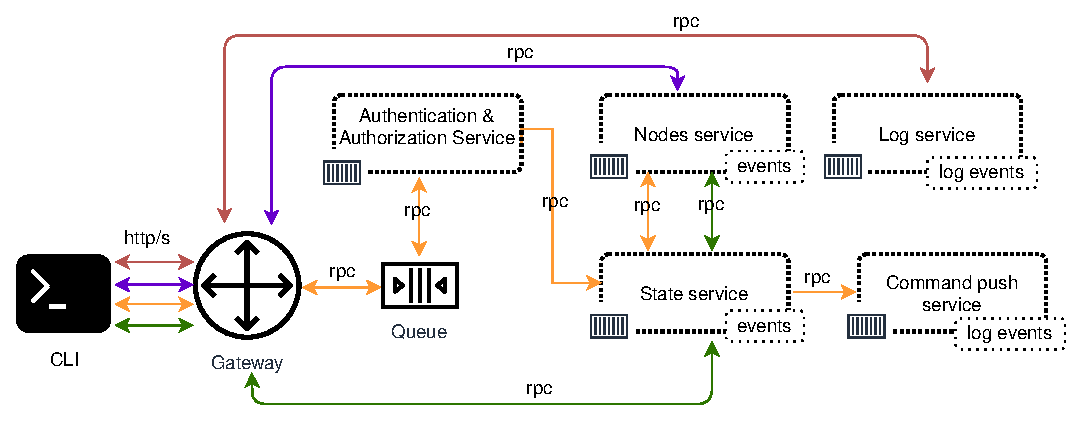
\includegraphics[width=\linewidth]{images/FIG5}
				\quickCite{Proof of concept implementation --- constellations project (c12s)}
			\end{center}
		\end{column}
	\end{columns}

\end{frame}

\begin{frame}
	\frametitle{Remote formation is tricky}
	
	\begin{itemize}
		\item Infrastructure deployment will not happen overnight -- it might take years
		\item It might not be started at all until the whole process is \emph{trivial} -- \textbf{simplify micro clouds management}
		\item The naive approach is doing it manually -- super tedious and time-consuming
		\item \textbf{The infrastructure needs to be constantly deployed and maintained} -- automation
		\item Prevent configuration drift -- the systems become different over time
	\end{itemize}
	
\end{frame}

\begin{frame}
	\frametitle{Then how?}
	
	\begin{itemize}
		\item It would be beneficial to view the \textbf{infrastructure as software} -- already available tools, principles, and techniques
		\item Model is \textbf{movable} in between edge and cloud, do we want more cloud-like or edge-like system
		\item Such \textbf{elasticity} requires infrastructure abstraction to the software level -- \textbf{infrastructure programming}
		\item This allow micro clouds infrastructure to be managed similarly as the software is
		\item Infrastructure definition is versioned, automated, and applied repeatedly and consistently every time -- \textbf{minimize configuration drift}
	\end{itemize}
	
\end{frame}

\begin{frame}
	\frametitle{Infrastructure programming artifacts}
	
	\begin{columns}
		\begin{column}{0.5\linewidth}
			\begin{itemize}
				\item Specify desired state using \emph{YAML} or some other format (descriptively)
				\item Submit \textbf{new state} to the system, and \textbf{let the system deal with the rest}
				\item \textbf{Immutable infrastructure deployment} allows for rolling update strategy -- updates large environments, a few nodes at the time
				\item Rely on containers for everything, even OS (LinuxKit)
				\item Sorry \textbf{no} DSLs here
			\end{itemize}
		\end{column}
		\begin{column}{0.5\linewidth}
			\includegraphics[width=\linewidth]{images/kelsie}\\
			\quickCite{Source: Twitter}
		\end{column}
	\end{columns}
	
\end{frame}

\begin{frame}
	\frametitle{The reconciler pattern}
	
	\begin{columns}
		\begin{column}{0.5\linewidth}
			\begin{itemize}
				\item System is dealing with changes using the \textbf{reconciler pattern}
				\item Track resources using two simple states:
				\begin{enumerate}
					\item \textbf{expected state} -- desired state
					\item \textbf{current state} -- actual state
				\end{enumerate}
				\item \textbf{Reconciliation loop} ensures that the desired state is maintained
				\item Every node must provide their current state -- \textbf{health-check} protocol
				\item Extension is simple
			\end{itemize}
		\end{column}
		\begin{column}{0.5\linewidth}
			\begin{center}
				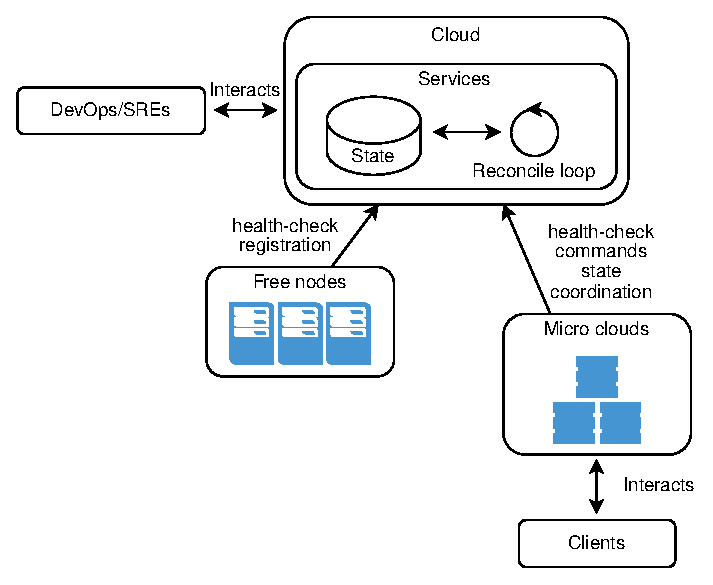
\includegraphics[scale=0.6]{images/Figure3}
			\end{center}
		\end{column}
	\end{columns}
	
\end{frame}

\begin{frame}
	\frametitle{What exists?}
	
	\begin{itemize}
		\item The existing orchestrator engines operate on a cluster level --- "treating \textbf{servers} as cattle, not pets" (i.e. numerous \textbf{servers} built using automated tools designed for failure, where no \textbf{server} is irreplaceable) --- cluster could span over multiple availability zones
		\item Kubernetes allows multi-cluster deployments, handling these clusters as disposable --- "treating \textbf{clusters} as cattle, not pets" (i.e., numerous \textbf{clusters} built using automated tools designed for failure, where no \textbf{clusters} are irreplaceable)
	\end{itemize}
	
\end{frame}

\begin{frame}
	\frametitle{And what's new -- challenging the state of the art?}
	
	\begin{itemize}
		\item This research goes one step further, allowing the creation of numerous micro clouds as disposable, using automated tools where no micro cloud is irreplaceable --- "treating \textbf{micro clouds} as cattle, not pets" (i.e. numerous \textbf{micro clouds} built using automated tools designed for failure, where no \textbf{micro cloud} is irreplaceable)
		\item More dimensions for operation and optimization of infrastructure and services
	\end{itemize}
	
\end{frame}

\begin{frame}
	\frametitle{Limitations}
	
	\begin{itemize}
		\item Specialized models are developed and optimized for a specific use case to take the maximum out of hardware and software
		\item They might outperform the proposed model in terms of speed
		\item The proposed model allows organization and reorganization of resources in a similar way the cloud does, allowing users to develop applications without some specialized infrastructure for different applications --- more development freedom
		\item Users will be able to create new interesting human-centered applications in the future, utilizing both cloud and edge
		\item The proposed model is more oriented towards developing a broader specter of applications without the need for a specialized hardware or software
	\end{itemize}
\end{frame}

\section{Applications}%
\subsection{Applications}%

\begin{frame}
	\frametitle{Applications}
	
	\begin{columns}
		\begin{column}{0.5\linewidth}
			
			\begin{itemize}
				\item All existing applications in the cloud can be upgraded to use the new model
				\item Big data applications \textbf{AND/OR} smart-sized, “data-centric” solutions to big issues -- Andrew Ng
				\item Real-time processing for proper decision making
				\item Eventually -- OS capable of running infrastructure without intervention
			\end{itemize}
			
		\end{column}
		\begin{column}{0.5\linewidth}
			\begin{center}
				\includegraphics[width=0.8\linewidth]{images/Figure29}
			\end{center}
		\end{column}
	\end{columns}
	
\end{frame}

\begin{frame}
	\frametitle{Use cases}
	
	\begin{center}
		\includegraphics[scale=0.4]{images/Figure25}
	\end{center}

\end{frame}

%\section{Future work}%
%\subsection{Future work}%

\section{Conclusion}%
\subsection{Conclusion}%

%\section{Conclusion}%
%\subsection{Conclusion}%

\begin{frame}
	\frametitle{Concluding remarks}

	\begin{center}
		The dynamic organization of geo-distributed nodes into micro clouds, forming distributed clouds
	\end{center}
	
	
	\bigskip
	Our model:
	\begin{itemize}
		\item Nodes are organized into micro clouds dynamically -- inspired by the cloud architecture
		\item Creation of numerous micro clouds designed for failure using automated tools where no micro cloud is irreplaceable -- "treating \textbf{micro clouds} as cattle, not pets."
		\item Serving local requests first
		\item Serving requests from optimal location
	\end{itemize} 
	
	\bigskip
	\begin{center}
		\HLight{"Containers are great, let’s run them everywhere." -- Brian Dorsey, Google Cloud Platform.}
	\end{center}
\end{frame}

\begin{frame}
	\frametitle{Future work}
	
	\begin{itemize}
		\item We barely scratched the surface, and there is still a lot of work to do
		\begin{itemize}
			\item Remote configurations and secrets management -- work in progress
			\item Hierarchical idempotence -- work in progress
			\item Namespaces and virtual clusters -- work in progresss
			\item Autoscaling -- scale everywhere
			\item File system/storage layer -- write once store everywhere
			\item Security aspects -- Security as code
			\item Applications framework
			\item Integration with existing infrastructure
			\item Lambda++ architecture
			\item Scheduling
			\item Chaos engineering 
			\item Monitoring
			\item etc.
		\end{itemize}
		\item  Not lacking opportunities
	\end{itemize}
	
\end{frame}

%\section{Questions}%
%\subsection{Questions}%

\begin{frame}
	
	\begin{center}
		\begin{Huge}
			Thank you for your attention!
		\end{Huge}
	\end{center}
	
\end{frame}
%%%%%%%%%%%%%%%%%%%%%%%%%%%%%%%%%%%

\end{document}
